\section{Auswertung}
\label{sec:Auswertung}

% Kurzer Text zur Fehlerfortpflanzung nach Gauss
Alle Fehler werden im Folgenden mit der Gaußschen Fehlerfortpflanzung berechnet.
Die Formel für abgeleitete Größen ist gegeben durch
\begin{equation*}
    \label{eqn:gauss}
    \Delta f = \sqrt{\sum_{i=1}^N \left( \frac{\partial f}{\partial x_i} \right)^2 \cdot (\Delta x_i)^2}.
\end{equation*}

\subsection{Vermessung des Acrylblocks mit Schieblehre}
\label{subsec:Schieblehre}


\begin{table}[!ht]
    \centering
    \caption{Ausmessung der Löcher im Acrylblock mit einer Schieblehre.}
    \begin{tabular}{|c|c|c|c|}
        \toprule
        {Loch} & {Abstand oben / mm} & {Abstand unten / mm} & {d / mm} \\
        \midrule
        1 & 59.00 \pm\, 0.04 & 19.10 \pm\, 0.04 & - \\
        2 & 60.82 \pm\, 0.04 & 17.46 \pm\, 0.04 & - \\
        3 & 13.08 \pm\, 0.04 & 60.64 \pm\, 0.04 & 5.92 \pm 0.06\\
        4 & 21.70 \pm\, 0.04 & 53.06 \pm\, 0.04 & 5.00 \pm 0.06\\
        5 & 30.26 \pm\, 0.04 & 45.46 \pm\, 0.04 & 3.92 \pm 0.06\\
        6 & 38.66 \pm\, 0.04 & 37.90 \pm\, 0.04 & 3.10 \pm 0.06\\
        7 & 46.70 \pm\, 0.04 & 29.86 \pm\, 0.04 & 3.10 \pm 0.06\\
        8 & 54.64 \pm\, 0.04 & 21.86 \pm\, 0.04 & 3.06 \pm 0.06\\
        9 & 62.70 \pm\, 0.04 & 13.70 \pm\, 0.04 & 3.04 \pm 0.06\\
        10 & 70.64 \pm\, 0.04 & 05.78 \pm\, 0.04 & 3.10 \pm 0.06\\
        11 & 15.20 \pm\, 0.04 & 54.24 \pm\, 0.04 & 10.00 \pm 0.06\\
        \bottomrule
    \end{tabular}
    \label{tab:Schieblehre}
\end{table}

Zur Bestimmung der Schallgeschwindigkeit %Und weitern Sachen?
wird der Acrylblock mit einer Schieblehre vermessen. Die Gesamthöhe des Blocks beträgt $h = \SI{79,76 \pm 0.04}{mm}.$
Die Messwerte sind in Tabelle \ref{tab:Schieblehre} aufgelistet.
Für alle Löcher wird der Abstand zur Ober- und Unterseite des Blocks gemessen.
Der Durchmesser der Löcher 3 bis 11 wird vermessen.
Die Durchmesser der Löcher 1 und 2 werden nicht weiter betrachtet, da sie zu klein sind um mit der Schieblehre vermessen zu werden.
Die Fehler der Messwerte werden mit $\Delta x = \SI{0,04}{mm}$ angenommen, was zwei Nonius-Einheiten entspricht.
Der Fehler für die Vermessung des Durchmessers wird etwas größer angenommen, da das genaue Ansetzen der Schieblehre nicht immer möglich war.


\subsection{Bestimmung der Schallgeschwindigkeit in Acryl}
\label{sec:Schallgeschwindigkeit}

% Grafik build/AkrylGeschwindigkeit.pdf einfuegen
\begin{figure}[!ht]
    \centering
    \includegraphics[width=\textwidth]{build/AcrylGeschwindigkeit.pdf}
    \caption{Bestimmung der Schallgeschwindigkeit in Acryl.}
    \label{fig:AkryllGeschwindigkeit}
\end{figure}

\begin{table}
    \centering
    \begin{tabular}{|c|c|c|}
        \toprule
        {Lochnummer} & {Laufzeit / µs} & {Höhe / mm} \\
        \midrule
        3 & 45.4 & 60.64\\
        4 & 39.5 & 53.06\\
        5 & 34.2 & 45.46\\
        6 & 28.6 & 37.90\\
        7 & 22.6 & 29.86\\
        8 & 19.6 & 21.86\\
        9 & 11.1 & 13.70\\
        11 & 40.4 & 54.24\\
        \bottomrule
    \end{tabular}\
    \caption{Laufzeiten und Höhen der Löcher 3 bis 11.}
    \label{tab:Schallgeschwindigkeit}
\end{table}

Zur Bestimmung der Schallgeschwindigkeit in Acryl werden die Laufzeiten zu sieben Löchern gemessen und gegen
die Höhe der Löcher aufgetragen. Die Schallgeschwindigkeit wird dann aus der Steigung der Ausgleichsgeraden bestimmt.
Die Dicke der Anpassungsschicht entspricht der Verschiebung der Ausgleichsgeraden in der y-Richtung.
Die Messwerte sind in Tabelle \ref{tab:Schallgeschwindigkeit} aufgelistet.
Die Ausgleichsgerade der Form $m\cdot x + b$ wird mit Python berechnet und ist in Abbildung \ref{fig:AkryllGeschwindigkeit} dargestellt.
So ergibt sich für die Schallgeschwindigkeit in Acryl
%Steigung:  2824.9278245842556 ± 84.76627810736713
%y-Achsenabschnitt:  -0.0030310985534149383 ± 0.0013618201193985383
\begin{equation*}
    m = c_\text{Acryl} = \SI{2824(84.7)}{\meter\per\second}
\end{equation*}
und für die Dicke der Anpassungsschicht
\begin{equation*}
    b = \SI{-0.0030(0.0014)}{\meter}.
\end{equation*}

\subsection{Bestimmung der Lage und Größe aller Fehlstellen mit dem Impuls-Echo-Verfahren}
\label{sec:ImpulsEcho}

\begin{table}
    \centering
    \caption{Tiefe der Löcher 3 bis 11 mit dem Impuls-Echo-Verfahren gemessen.}
    \begin{tabular}{|c|c|c|}
        \toprule
        {Loch} & {Depth oben / mm} & {Depth unten / mm} \\
        \midrule
        3 & 14.3 & 61.2\\
        4 & 22.4 & 54.0\\
        5 & 31.1 & 46.5\\
        6 & 39.4 & 39.2\\
        7 & 48.1 & 30.8\\
        8 & 55.5 & 22.8\\
        9 & 63.6 & 15.2\\
        10 & 72.1 & 07.2\\
        11 & 16.4 & 55.4\\
        \bottomrule
    \end{tabular}
    \label{tab:ImpulsEchoTiefe}
\end{table}

Um die genaue Lage und Größe der Fehlstellen zu bestimmen, wird im Messprogramm auf die \textbf{Depth} Anzeigeeinstellung gewechselt.
Die Messwerte sind in Tabelle \ref{tab:ImpulsEchoTiefe} aufgelistet.
Die Gesamthöhe des Blocks wird mit
\begin{equation*}
    h = h_o + d + h_u - b = \SI{79,76 \pm 0.04}{mm},
\end{equation*}
mit $h_o$ als Höhe über, $h_u$ als Höhe unter und $d$ als Durchmesser der Fehlstellen.
Bei den mit Ultraschall gemessenen Werten muss  die Dicke der Anpassungsschicht $b$ abgezogen werden um korrekte Ergebnisse zu erhalten.

\begin{table}
    \centering
    \caption{Durchmesser der Löcher 3 bis 11 mit dem Impuls-Echo-Verfahren gemessen.}
    \begin{tabular}{|c|c|}
        \toprule
        {Loch} & {d / mm}\\
        \midrule
        3 & 7.3\pm \,1.4\\
        4 & 6.4\pm \,1.4\\
        5 & 5.2\pm \,1.4\\
        6 & 4.2\pm \,1.4\\
        7 & 3.9\pm \,1.4\\
        8 & 4.5\pm \,1.4\\
        9 & 4.0\pm \,1.4\\
        10 & 3.5\pm \,1.4\\
        11 & 11.0\pm \,1.4\\
        \bottomrule
    \end{tabular}
    \label{tab:ImpulsEchoDurchmesser}
\end{table}


\subsection{Untersuchung des Auflösungsvermögens}
\label{sec:Aufloesung}

% Grafiken einfuegen
\begin{figure}[H]
    \centering
    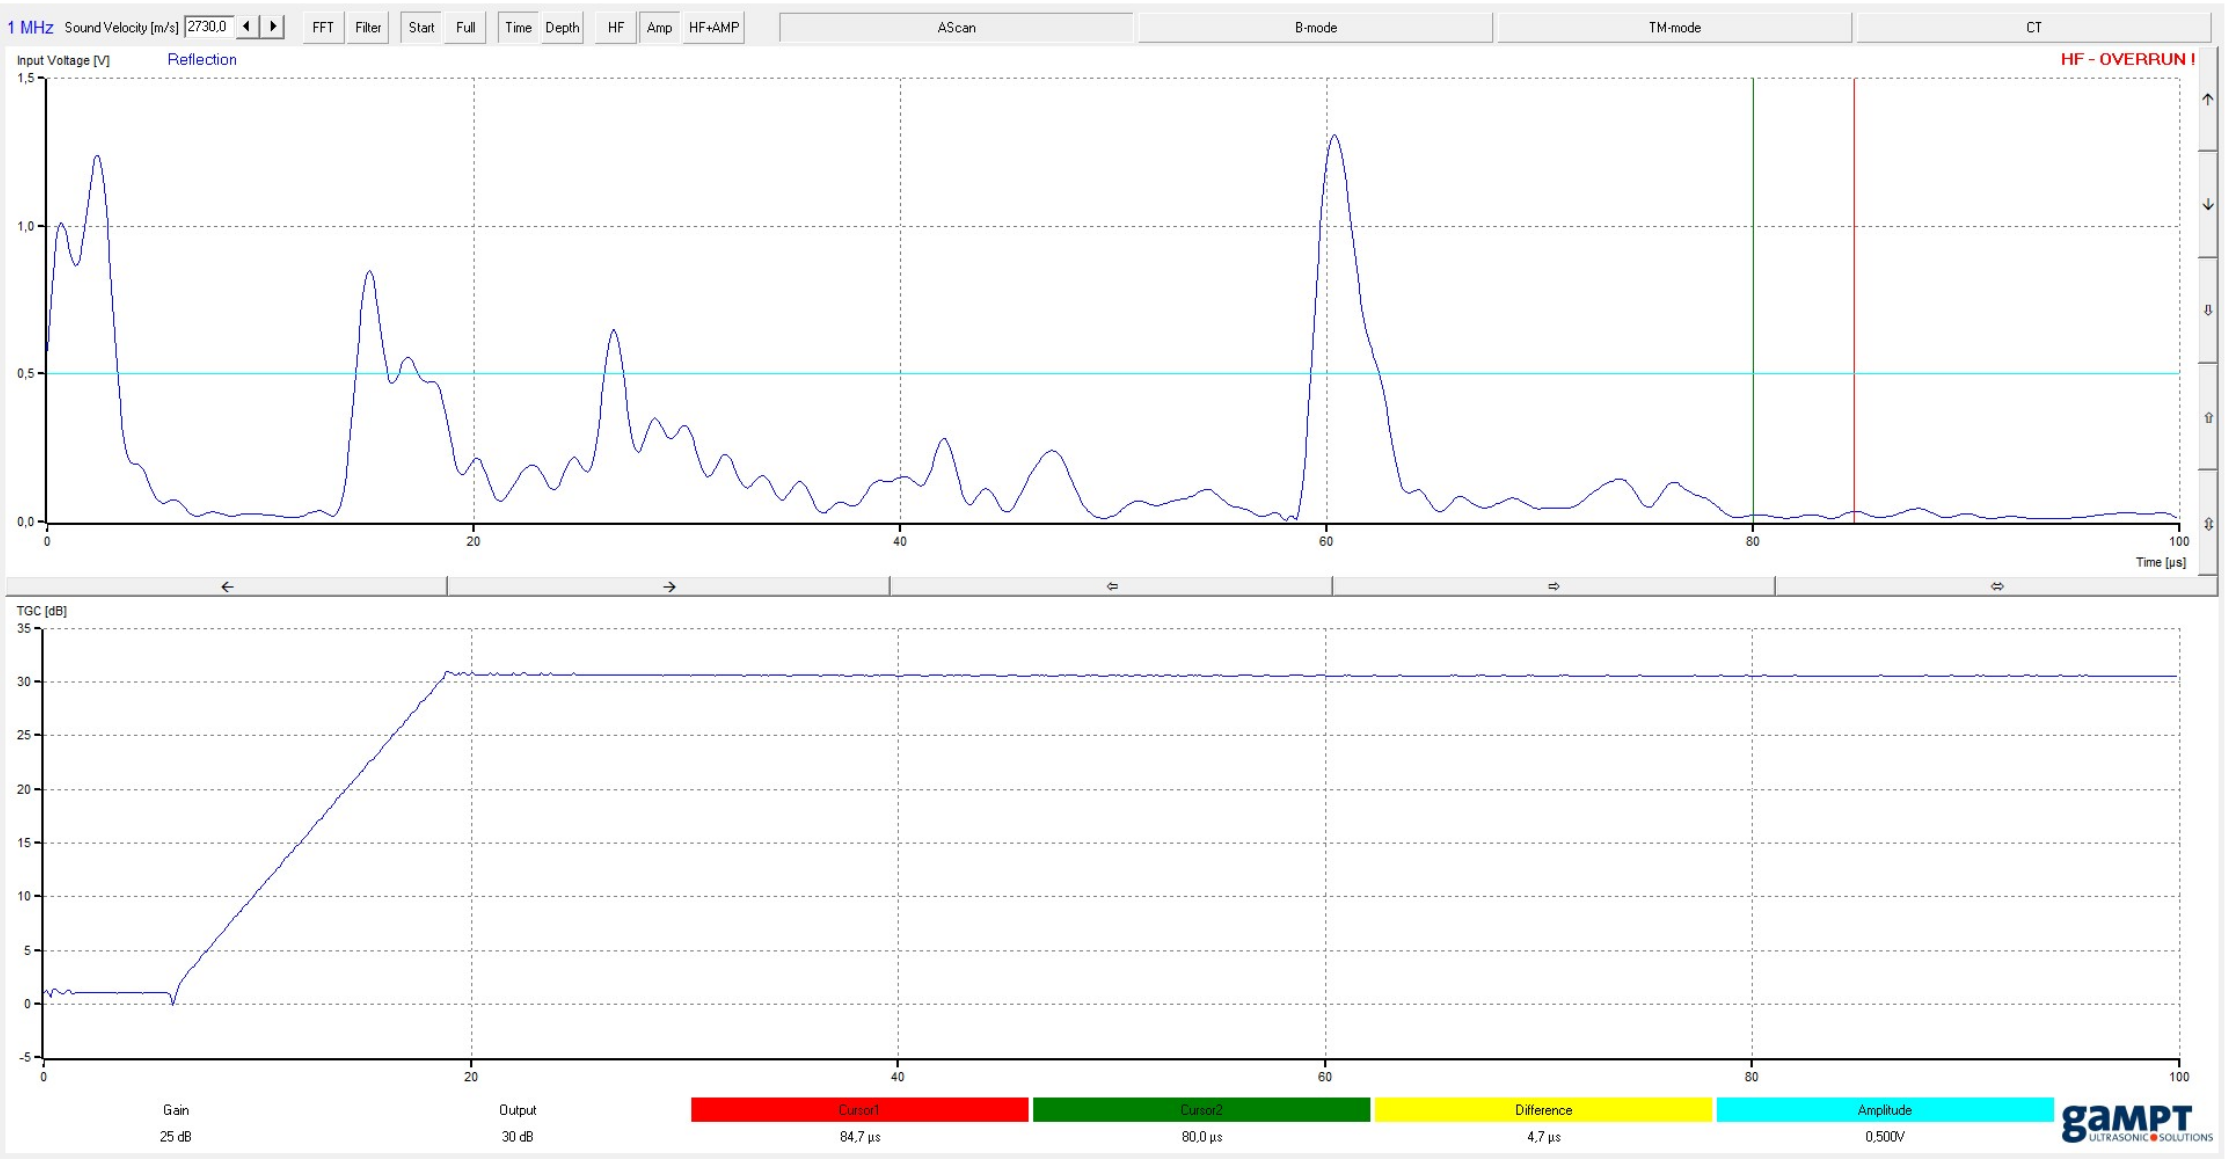
\includegraphics[width=\textwidth]{img/Aufloesung_1Mhz.png}
    \caption{Untersuchung des Auflösungsvermögens mit 1 Mhz Sonde.}
    \label{fig:Aufloesung1Mhz}
\end{figure}


\begin{figure}[H]
    \centering
    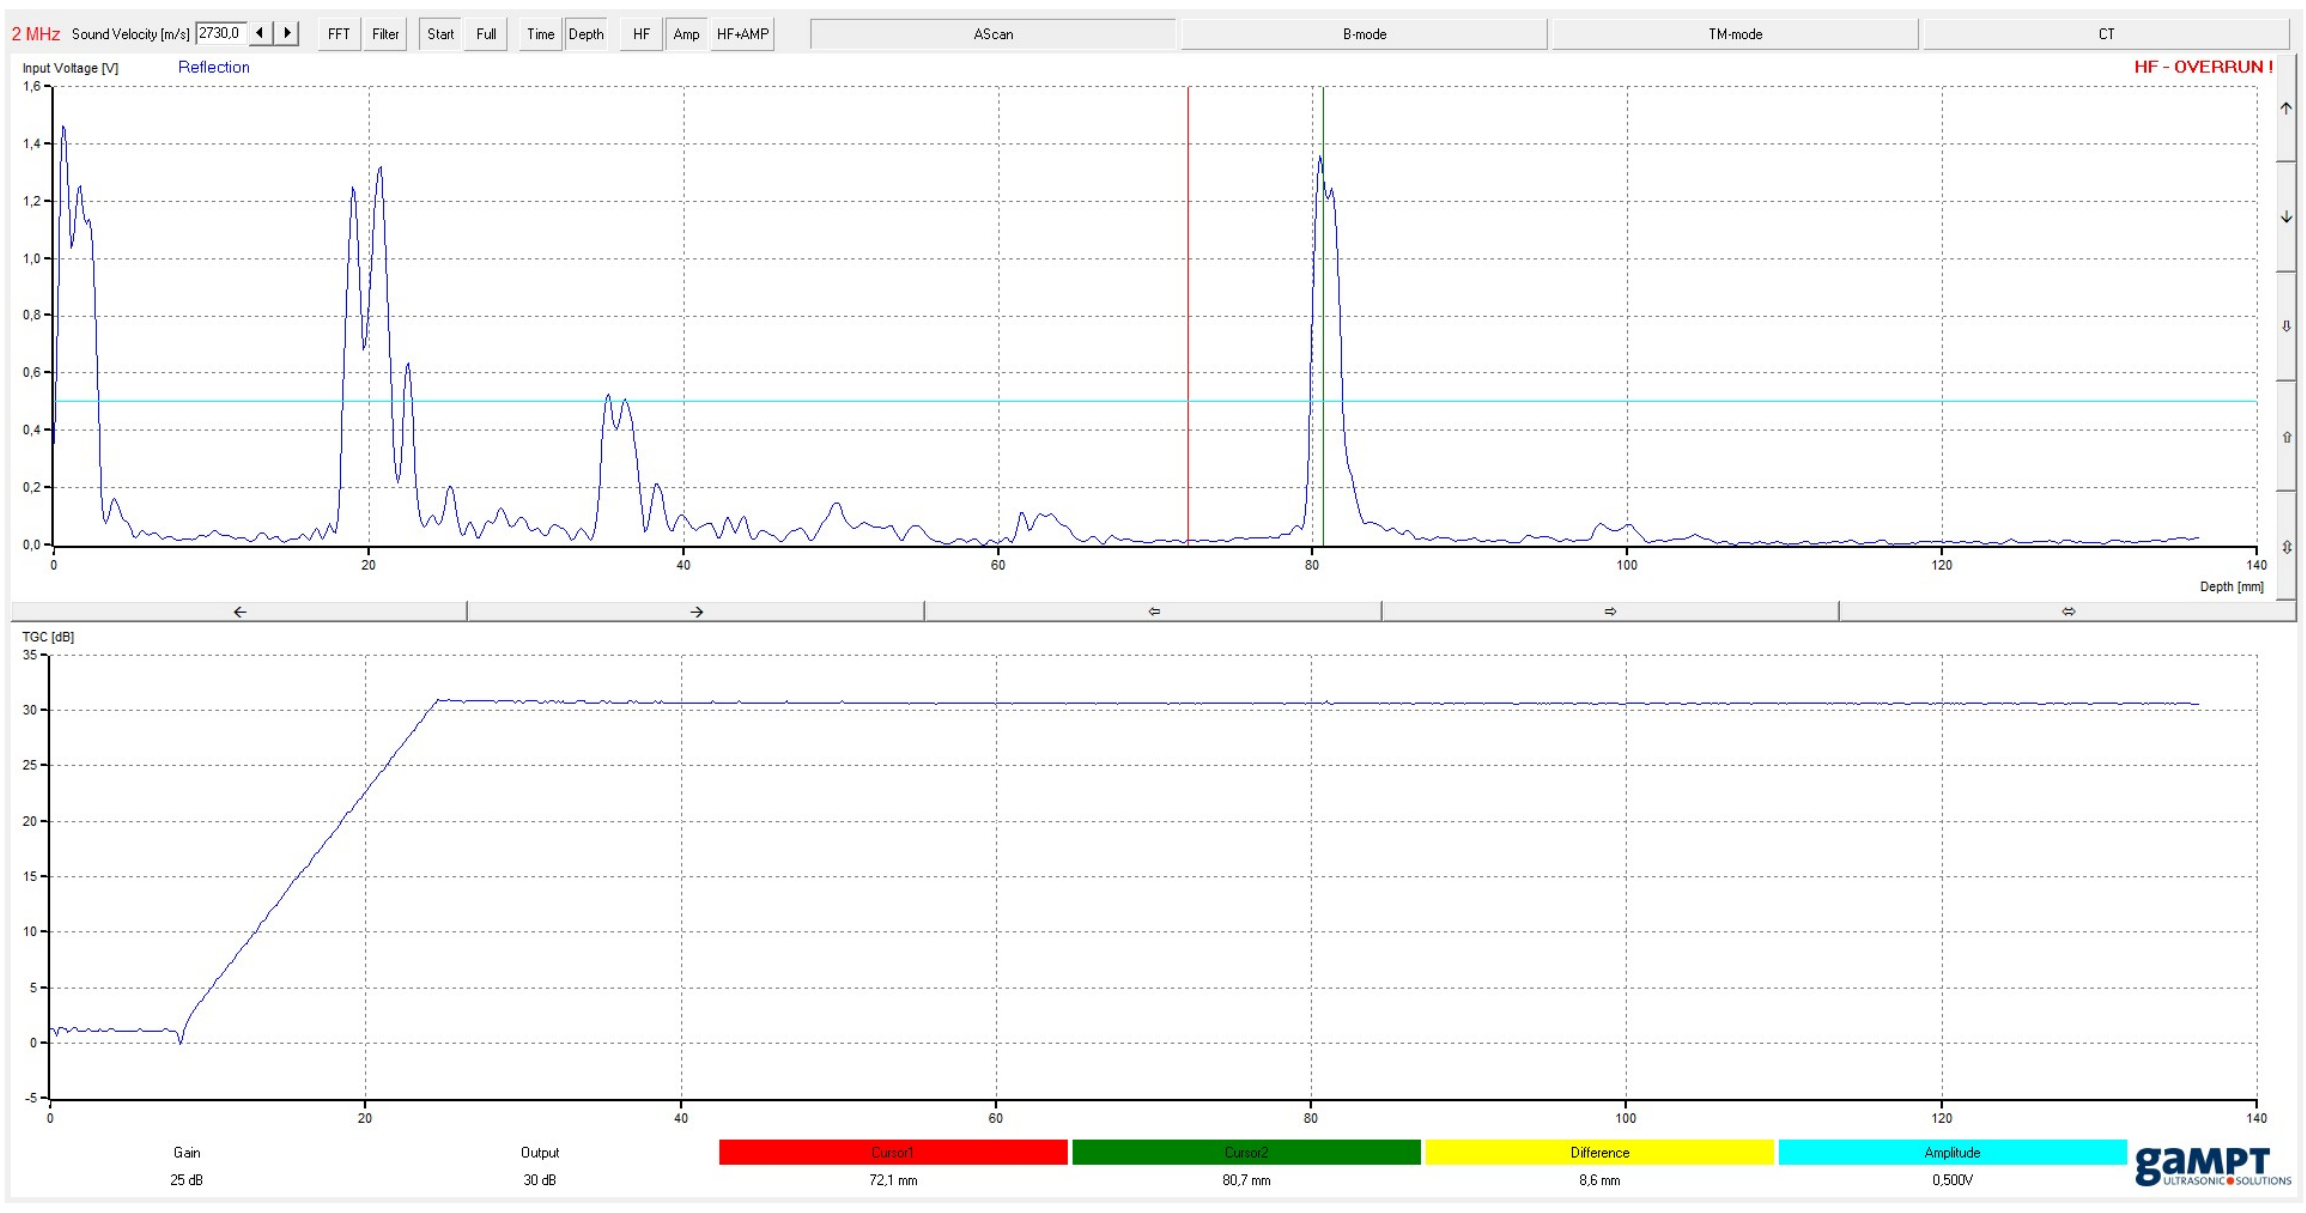
\includegraphics[width=\textwidth]{img/Aufloesung_2Mhz.png}
    \caption{Untersuchung des Auflösungsvermögens mit 2 Mhz Sonde.}
    \label{fig:Aufloesung2Mhz}
\end{figure}

Zur Untersuchung des Auflösungsvermögens werden die Sonden auf die Löcher 1 und 2 gerichtet.
Die Messungen sind in den Abbildungen \ref{fig:Aufloesung1Mhz} und \ref{fig:Aufloesung2Mhz} dargestellt.
Die mit der 1 Mhz Sonde gemessenen Peaks sind nicht zu unterscheiden, da sie sich überlagern.
Die Peaks der 2 Mhz Sonde sind unterscheidbar. 


\subsection{Untersuchung des Acrylblocks mit dem B-Scan}
\label{sec:BScanAcryl}

\begin{figure}
    \centering
    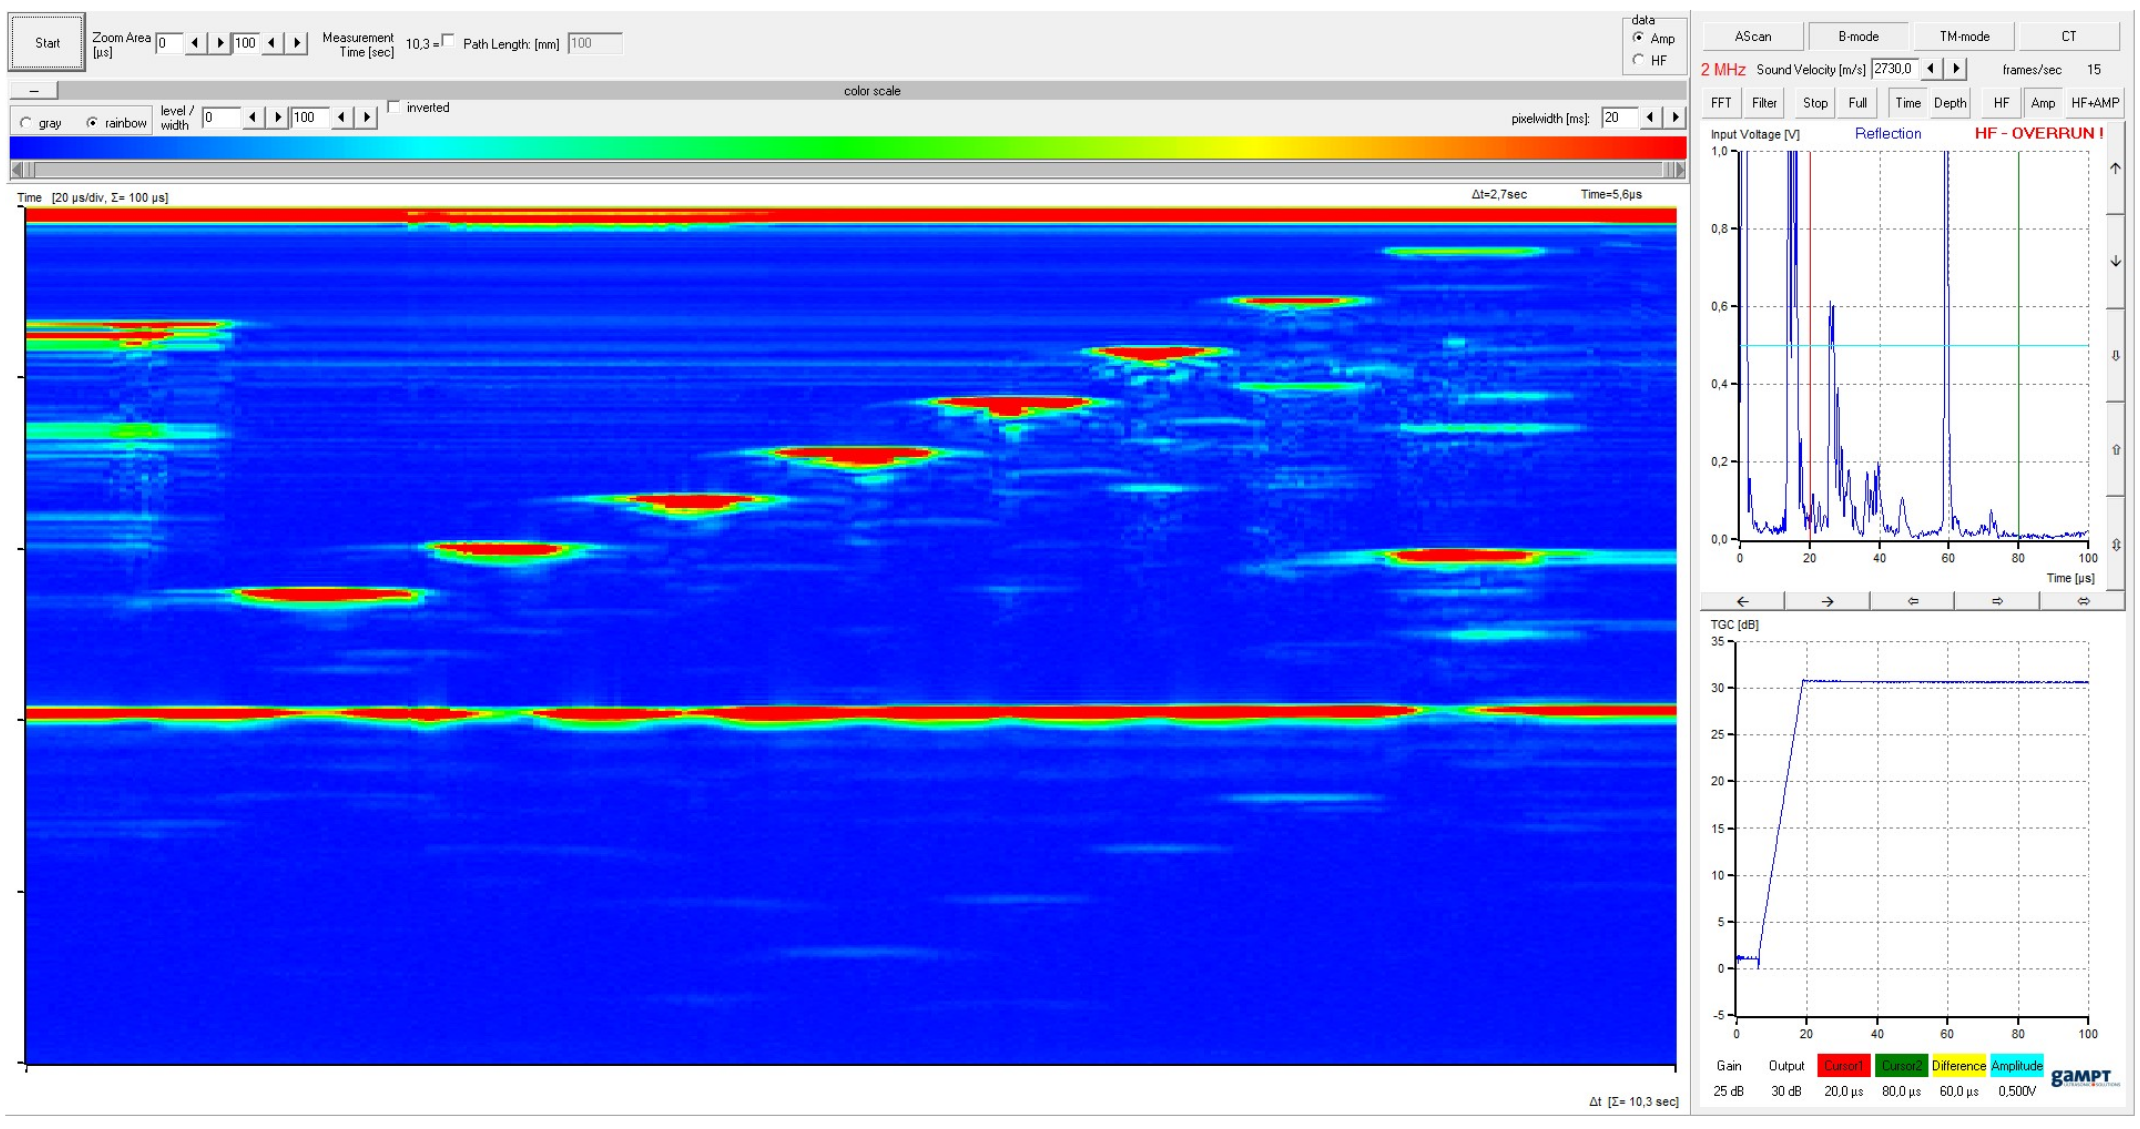
\includegraphics[width=0.9\textwidth]{img/b-scan2.png}
    \caption{B-Scan des Acrylblocks von der Oberseiteseite.}
    \label{fig:BScanSeiteOben}
\end{figure}

\begin{figure}
    \centering
    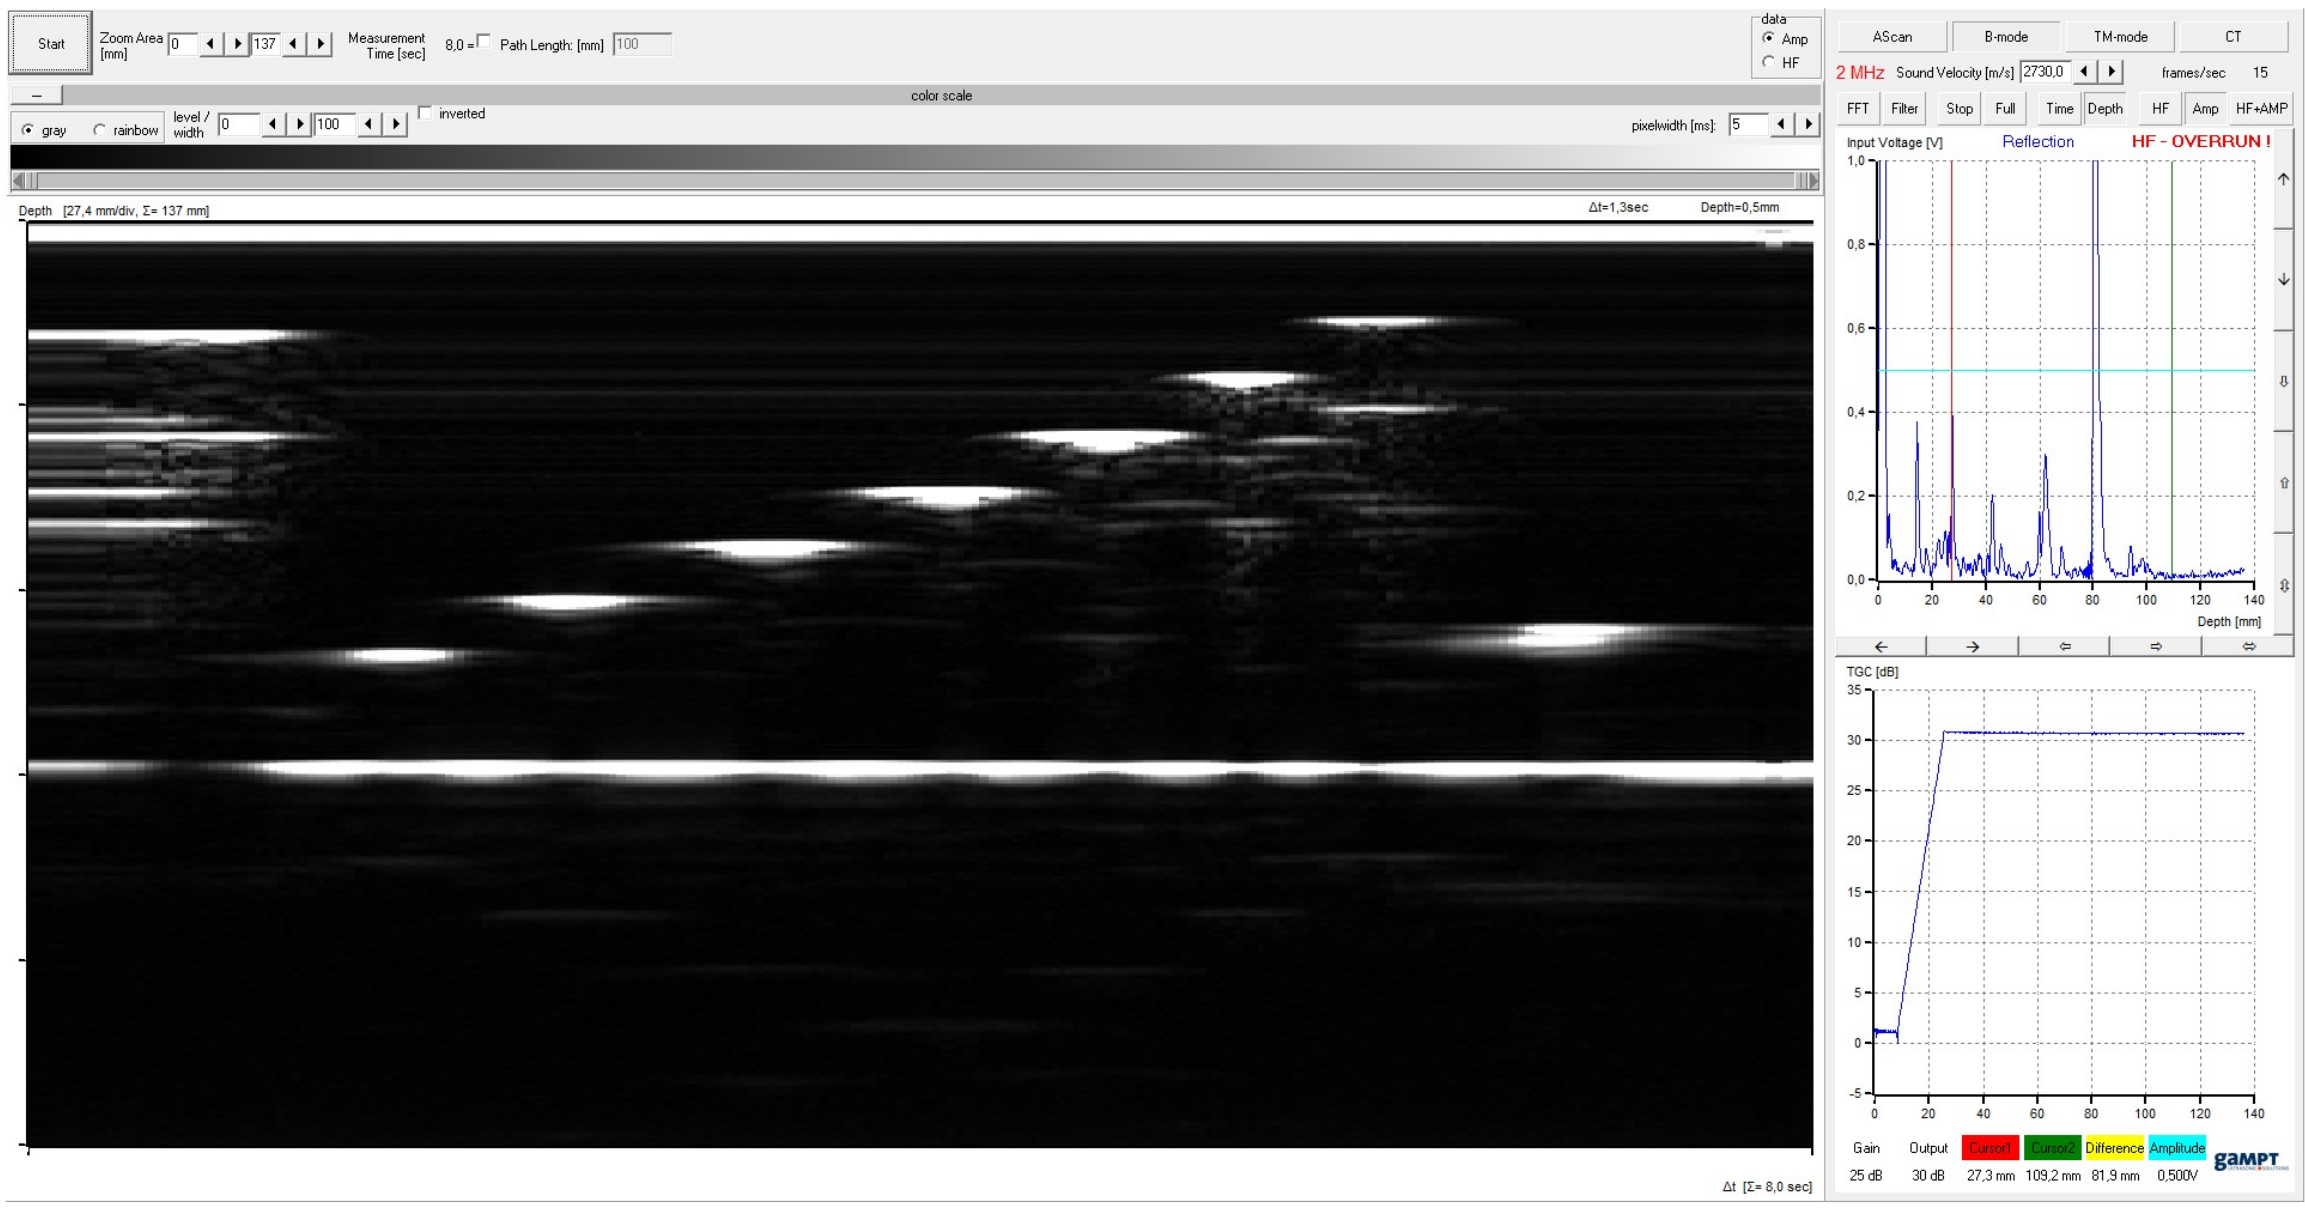
\includegraphics[width=0.9\textwidth]{img/b-scanunten1.png}
    \caption{B-Scan des Acrylblocks von der Unterseite.}
    \label{fig:BScanSeiteUnten}
\end{figure}

\begin{table}
    \centering
    \caption{Durchmesser der Löcher 3 bis 11 mit dem B-Scan-Verfahren gemessen.}
    \begin{tabular}{|c|c|c|c|}
        \toprule
        {Loch} & {Oberseite / mm} & {Unterseite / mm} & {d / mm}\\
        \midrule
        3 & 44.8 & 14.5 & 23.5\pm \,1.4\\
        4 & 39.2 & 23.0 & 20.6\pm \,1.4\\
        5 & 33.6 & 31.7 & 17.5\pm \,1.4\\
        6 & 28.2 & 39.9 & 14.7\pm \,1.4\\
        7 & 22.4 & 47.9 & 12.5\pm \,1.4\\
        8 & 16.6 & 57.8 & 8.4\pm \,1.4\\
        9 & 10.7 & 63.6 & 8.5\pm \,1.4\\
        11 & 40.0 & 16.7 & 26.1\pm \,1.4\\        
        \bottomrule        
    \end{tabular}
    \label{tab:BScanDurchmesser}
\end{table}

Mithilfe des Cursors wird die Lage der Störstellen bestimmt.
Die Durchmesser der Störstellen werden wieder wie in \autoref{sec:ImpulsEcho} berechnet.
Die Ergebnisse sind in Tabelle \ref{tab:BScanDurchmesser} aufgelistet.
Für Loch 10 ist kein Durchmesser angegeben, da es nicht auf dem B-Scan zu sehen ist.
Die mit dem B-Scan ermittelten Durchmesser liegen weiter von den mit der Schieblehre aufgenommenen Werten entfernt als die mit dem A-Scan ermittelten.

\subsection{Untersuchung Brustmodells mit dem B-Scan}
\label{sec:BScanBrust}

\begin{figure}
    \centering
    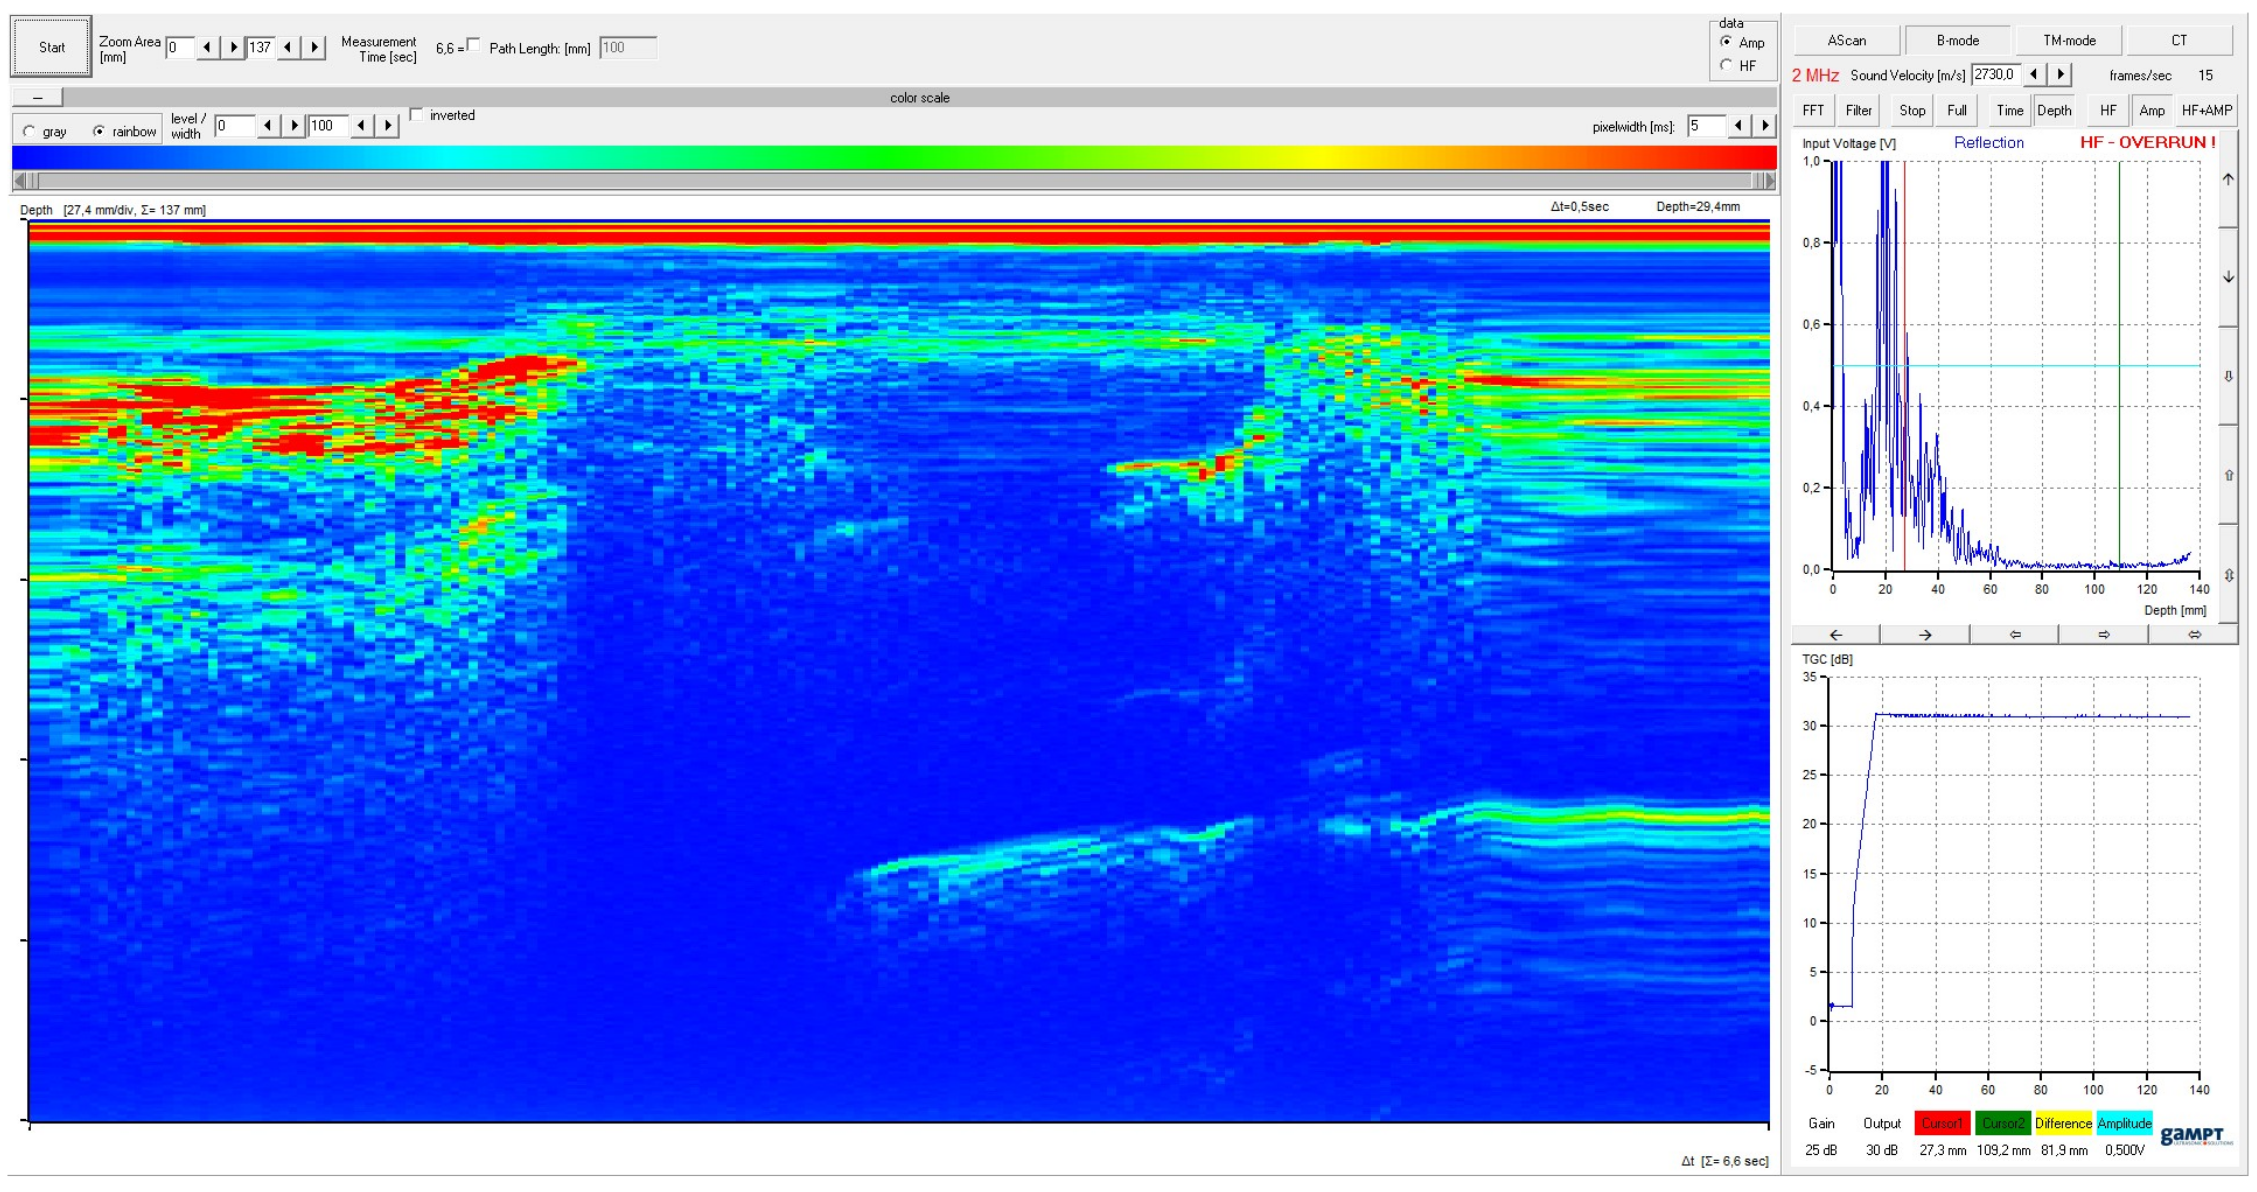
\includegraphics[width=0.9\textwidth]{img/BrustB-Scan.png}
    \caption{B-Scan des Brustmodells zur Tumorbestimmung.}
    \label{fig:BScanBrust}
\end{figure}

Der auf der linken Seite der Abbildung \ref{fig:BScanBrust} zu sehende Tumor hat eine größere Ausdehnung als der auf der rechten Seite.
Der größere Tumor zeichnet sich klarer ab, was darauf hindeutet, dass die Schallwellen an der Grenzfläche zwischen Tumor und Gewebe stärker reflektiert werden.
Es handelt sich also vermutlich um festes Gewebe und so um einen bösartigen Tumor.
Der kleinere Tumor ist schlechter zu sehen. Dies deutet darauf hin, dass die Schallwellen an der Grenzfläche zwischen Tumor und Gewebe weniger stark reflektiert werden.
Vermutlich handelt es sich um eine Flüssigkeitsansammlung und so um einen gutartigen Tumor.
Der größere Tumor liegt weiter unten auf dem Scan und somit auch tiefer in der Brust.